
\newpage
\section{Chapter 5 - Convergence of Random Variables}

\medskip\noindent\textbf{Definition 5.1} Types of convergence\\
Let $X_1,X_2,\ldots$ be a sequence of random variables and let $X$ be another
random variable. Let $F_n$ denote the CDF of $X_n$ and let $F$ denote the CDF of $X$.

\medskip\noindent
1. $X_n$ converges to $X$ in \emph{probability}, $X_n\raP X$, if for all $\epsilon > 0$,
$$
\P(|X_n - X| > \eps)\ra 0
$$
as $n\ra\infty$.

\medskip\noindent
2. $X_n$ converges to $X$ in \emph{distribution}, $X_n\raD X$, if
$$
\lim_{n\ra\infty}F_n(t) = F(t)
$$
at all $t$ for which $F$ is continuous.

\medskip\noindent\textbf{Definition 5.2}\\
$X_n$ converges to $X$ in \emph{quadratic mean} ($L_2$), written $X_n\raQ X$, if
$$
\E[(X_n - X)^2]\ra 0
$$
as $n\ra\infty$.

\medskip\noindent
Relationship in convergence types.
$$
\raQ \imp \raP \imp \raD
$$

\subsection*{Exercises}
%%%%%%%%%%%%%%%%%%%%%%%%%%%%%%%%%%%%%%%%%%%%%%%%%%%%%%%%%%%%%%%%%%%%%%%%%%%%%%%
\textbf{5.1}\\  % PDF page 82
Let $X_1,\ldots, X_n$ be IID with finite mean and variance $\mu$ and $\sigma^2$.
Let $\bar{X}$ be the sample mean and $S_n^2$ be the sample variance.
$$
\bar{X} = \frac{1}{n}\sum_{i=1}^n,
\qquad
S_n^2 = \frac{1}{n-1}\sum_{i=1}^n(X_i - \bar{X})^2
$$

\medskip\noindent(a) Showing that $\E[S_n^2] = \sigma^2$ was done in exercise 3.8.

\medskip\noindent(b) Showing that $S_n^2\raP\sigma^2$. Directly, this means that for any $\eps>0$,
$$
\P(|S_n^2 - \sigma^2| > \eps) = 0 \;\;\text{as}\;\; n\ra\infty.
$$
But we can do it in a different way. Following the hint, we want to rewrite $S_n^2$
so we can apply the law of large numbers.

\medskip\noindent
Doing the calculations on the next page.

\newpage\noindent
\begin{align*}
    S_n^2 &= \frac{1}{n-1}\sum_{i=1}^n(X_i - \bar{X})^2 \\
    &= \frac{n}{n-1}\left(\frac{1}{n}\sum_{i=1}^n\Big[X_i^2 - 2X_i\bar{X} + \bar{X}^2\Big]\right) \\
    \shortintertext{Distributing the sum.}
    &= \frac{n}{n-1}\left(\frac{1}{n}\sum_{i=1}^nX_i^2 - 2\bar{X}\left(\frac{1}{n}\sum_{i=1}^n X_i\right) + \bar{X}^2\right) \\
    &= \frac{n}{n-1}\left(\frac{1}{n}\sum_{i=1}^nX_i^2 - 2\bar{X}^2 + \bar{X}^2\right) \\
    &= \frac{n}{n-1}\left(\frac{1}{n}\sum_{i=1}^nX_i^2 - \bar{X}^2\right) \\
    \shortintertext{WLLN on $\bar{X}^2$ with $g(x) = x^2$.}
    &= \frac{n}{n-1}\left(\frac{1}{n}\sum_{i=1}^nX_i^2 - \mu^2\right) \\
    &= \frac{n}{n-1}\left(\frac{1}{n}\sum_{i=1}^n(X_i - \mu)^2\right)
\end{align*}
The last rewrite is a standard identity. Now, we define $Y_i = X_i - \mu$. Then
$\bar{Y} \ra \E[(X_i - \mu)]$ by the WLLN. By Theorem 5.5(f), we can apply $g(x) = x^2$
and get $\bar{Y}^2 \ra \E[(X_i - \mu)^2] = \V(X_i) = \sigma^2$. Finally, we use the hint
with $c_n = n/(n-1)$ which obviously tends to 1, so we can apply
Theorem 5.5(d) and hence we have proved that $S_n^2 \raP \sigma^2$. (The hint says using
5.5(e), but that is convergence with distribution, which I don't think is correct).
(Update: this is a misprint which is noted in the errata2.pdf for the book).

\bigskip\noindent
%%%%%%%%%%%%%%%%%%%%%%%%%%%%%%%%%%%%%%%%%%%%%%%%%%%%%%%%%%%%%%%%%%%%%%%%%%%%%%%
\textbf{5.2}\\  % PDF page 82
Let $X_1,X_2\ldots$ be a sequence of random variables. Show that $X_n \raQ b$
if and only if
$$
\lim_{n\ra\infty}\E[X_n] = b,
\quad\text{and}\quad
\lim_{n\ra\infty}\V[X_n] = 0.
$$
\textsc{Proof}.\\
$\Rightarrow$) We assume $X_n \raQ b$, which means
$$
\E[(X_n - b)^2]\ra 0,\quad n\ra\infty.
$$
We can rewrite the expression:
\begin{align*}
    \E[(X_n - b)^2] &= \E[X_n^2 - 2bX_n + b^2] \\
    &= \E[X_n^2] - 2b\E[X_n] + b^2 \\
    &= \E[X_n^2] - \E[X_n]^2 + \E[X_n]^2 - 2b\E[X_n] + b^2 \\
    &= \V(X_n) + (\E[X_n] - b)^2
\end{align*}

\newpage\noindent
By our assumption $\E[(X_n - b)^2]\ra 0$ as $n\ra\infty$, and so 
$\V(X_n) + (\E[X_n] - b)^2 \ra 0$ as $n\ra\infty$.
Since $\V(X_n) \geq 0$ and $(\E[X_n] - b)^2 \geq 0$, then we can conclude that
$$
\V(X_n) \ra 0,
\qquad
(\E[X_n] - b)^2 \ra 0 \imp \E[X_n] \ra b
$$
as $n\ra\infty$.\\
$\Leftarrow$) We assume 
$$
\lim_{n\ra\infty}\E[X_n] = b,
\quad\text{and}\quad
\lim_{n\ra\infty}\V[X_n] = 0.
$$
Then $\lim_{n\ra\infty} \V(X_n) + (\E[X_n] - b)^2 = 0$.
By reversing the calculations from the first part:
$$
\lim_{n\ra\infty} \V(X_n) + (\E[X_n] - b)^2 = 0
\imp
\lim_{n\ra\infty} \E[(X_n - b)^2] = 0
\imp
X_n \raQ b.
$$
By showing implication both ways, the result is proved.\qed

\bigskip\noindent
%%%%%%%%%%%%%%%%%%%%%%%%%%%%%%%%%%%%%%%%%%%%%%%%%%%%%%%%%%%%%%%%%%%%%%%%%%%%%%%
\textbf{5.3}\\  % PDF page 83
Let $X_1,\ldots, X_n$ be IID and let $\mu = \E[X_i]$ with finite variance.
Show that $\bar{X} \raQ \mu$.

\medskip\noindent\textsc{Proof}. Define:
$$
\bar{X}_n = \frac{1}{n}\sum_{i=1}^n X_i.
$$
By the WLLN, $\bar{X}_n\raP \mu$, which we can also express as
$$
\lim_{n\ra\infty}\E[\bar{X}_n] = \mu.
$$
The variance is finite, so $\V(X_i) = \sigma^2 <\infty$. This means that for
the sample variance:
$$
\lim_{n\ra\infty} \V(\bar{X}) = \lim_{n\ra\infty} \frac{\sigma^2}{n} = 0.
$$
With this, we can simply apply the result from exercise 5.2 which shows that
$\E[(\bar{X} - \mu)^2]\ra 0$ as $n\ra\infty$ which proves $\bar{X}\raQ \mu$.\qed

\bigskip\noindent
%%%%%%%%%%%%%%%%%%%%%%%%%%%%%%%%%%%%%%%%%%%%%%%%%%%%%%%%%%%%%%%%%%%%%%%%%%%%%%%
\textbf{5.4}\\  % PDF page 83
Let $X_1,X_2,\ldots$ be a sequence of random variables such that
$$
\P\left(X_n = \frac{1}{n}\right) = 1 - \frac{1}{n^2},
\quad\text{and}\quad
\P(X_n = n) = \frac{1}{n^2}.
$$
Just noting the probabilities for each outcome as $n$ grows.
$$
\begin{tabular}{l|l|l|l|l|l}
           &$n=1$&$n=2$&$n=3$&$n=4$&$\ldots$ \\
           \hline
\rule{0pt}{10pt}$p(x) = \P(X_n = \frac{1}{n})$ &$p(1) = 0$&$p(\frac{1}{2}) = \frac{3}{4}$&$p(\frac{1}{3}) = \frac{8}{9}$&$p(\frac{1}{4}) = \frac{15}{16}$&$\ldots$\\
\rule{0pt}{10pt}$p(x) = \P(X_n = n)$ &$p(1) = 1$&$p(2) = \frac{1}{4}$&$p(3) = \frac{1}{9}$&$p(4) = \frac{1}{16}$&$\ldots$\\
\hline
\end{tabular}
$$
As $n$ becomes large, the probability that we get $n$ and not $1/n$ becomes very small.
But as $n$ becomes large, it will also yield extreme outliers in the sequence with
a non-zero probability.

\newpage\noindent
Starting by calculating the mean, second moment, and variance.
\begin{align*}
    \E[X_n] &= \left(\frac{1}{n}\right)\left(1 - \frac{1}{n^2}\right) + (n)\left(\frac{1}{n^2}\right)\\
    &= \frac{1}{n} - \frac{1}{n^3} + \frac{1}{n} \\
    &= \frac{2}{n} - \frac{1}{n^3}
\end{align*}
\begin{align*}
    \E[X_n^2] &= \left(\frac{1}{n^2}\right)\left(1 - \frac{1}{n^2}\right) + (n^2)\left(\frac{1}{n^2}\right)\\
    &= \frac{1}{n^2} - \frac{1}{n^4} + 1
\end{align*}
\begin{align*}
    \V(X_n) &= \E[X_n^2] - \E[X_n]^2 \\
    &= \frac{1}{n^2} - \frac{1}{n^4} + 1 - \left(\frac{2}{n} - \frac{1}{n^3}\right)^2 \\
    &= \frac{1}{n^2} - \frac{1}{n^4} + 1 - \left(\frac{4}{n^2} - \frac{4}{n^4} + \frac{1}{n^6}\right) \\
    &= 1 - \frac{3}{n^2} + \frac{3}{n^4} - \frac{1}{n^6}
\end{align*}
Results verified by simulation. (See code in \texttt{5.4.R}). E.g. for $n=200$ and 10M simulations:
\begin{lstlisting}[style=RSyntax, title=R]
# Simulated vs. Theoretical
> mean(Xn)
[1] 0.009879878
> 2/n - 1/n^3
[1] 0.009999875
> var(Xn)
[1] 0.9759275
> 1 - 3/n^2 + 3/n^4 - 1/n^6
[1] 0.999925
\end{lstlisting}
From these expressions we can see that $\lim_{n\ra\infty} \E[X_n] = 0$, but $\lim_{n\ra\infty} \V(X_n) = 1$.
Since the variance does not become 0, we know by the result in exercise 5.2 that this does
NOT converge in quadratic mean.

Checking if $X_n$ converges in probability. If we fix some $\eps > 0$, we can apply
the Chebyshev inequality. Set $\mu = \E[X_n]$ and $\sigma^2 = \V(X_n)$:
$$
\P(|X_n -\mu| > \eps) \leq \frac{\sigma^2}{\eps^2}
= \frac{1 - \frac{3}{n^2} + \frac{3}{n^4} - \frac{1}{n^6}}{\eps^2}
$$
By taking the limit $n\ra\infty$ on both sides, we get:
$$
\lim_{n\ra\infty} \P(|X_n -\mu| > \eps)
\leq
\lim_{n\ra\infty} \frac{1 - \frac{3}{n^2} + \frac{3}{n^4} - \frac{1}{n^6}}{\eps^2}
= \frac{1}{\eps^2}.
$$
Since this does not tend to 0, we do NOT have convergence in probability.

\newpage\noindent
%%%%%%%%%%%%%%%%%%%%%%%%%%%%%%%%%%%%%%%%%%%%%%%%%%%%%%%%%%%%%%%%%%%%%%%%%%%%%%%
\textbf{5.5}\\  % PDF page 83
Let $X_1,\ldots,X_n\sim\text{Bernoulli}(p)$. Prove that
$$
\frac{1}{n}\sum_{i=1}^n X_i^2 \raP p,
\quad\text{and}\quad
\frac{1}{n}\sum_{i=1}^n X_i^2 \raQ p.
$$
\textsc{Proof}. Recalling how to calculate the expectation and second moment
for a Bernoulli$(p)$ variable:
$$
\E[X] = (1)p + (0)(p-1) = p,
\qquad
\E[X^2] = (1)^2p + (0)^2(p-1) = p,
$$
With these, we can calculate the variance.
$$
\V(X) = \E[X^2] - \E[X]^2 = p - p^2 = p(1 - p).
$$
%Since the $X_i$ are IID, we can apply the WLLN to establish that $\bar{X} \raP p$.
We define $Y_i := X_i^2$ and exploit the simplicity of the Bernoulli distribution.
In this case:
$$
\E[Y] = \E[X^2] = (1)^2p + (0)^2(p-1) = p,
\qquad
\E[Y^2] = \E[X^4] = (1)^4p + (0)^4(p-1) = p,
$$
With these, we can calculate the variance.
$$
\V(Y) = \E[Y^2] - \E[Y]^2 = p - p^2 = p(1 - p).
$$
So we have $\mu = \E[Y] = p$ and $\sigma^2 = p(1-p)$.
We can now define the sample mean and variance:
$$
\E[\bar{Y}] = p,\qquad \V(\bar{Y}) = \frac{\sigma^2}{n} = \frac{p(1 - p).}{n}.
$$
Since the variance tends to 0 as $n\ra\infty$ we can use the results in exercise 5.3
to conclude that $\bar{Y}\raQ p$ and by how we defined $Y$, $\frac{1}{n}\sum_{i=1}^n X_i^2 \raQ p$.
Since we have convergence in quadratic mean, it follows that we also have convergence
in probability. \qed

\bigskip\noindent
%%%%%%%%%%%%%%%%%%%%%%%%%%%%%%%%%%%%%%%%%%%%%%%%%%%%%%%%%%%%%%%%%%%%%%%%%%%%%%%
\textbf{5.6}\\  % PDF page 83
The height of men has mean 68 inches and standard deviation 2.6 inches. We have $n=100$.
Finding the approximate probability that the average height in the sample will
be at least 68 inches.

 We can approximate this probability with the CLT (central limit theorem). We want to
 find the probability that the sample height $\bar{X} = \frac{1}{n}\sum_{i=1}^n X_i$
 is at least as big as the population mean: $\P(\bar{X} > \mu)$. 
 $$
 \P(\bar{X} > \mu) =
 1 - \P(\bar{X} \leq \mu) %\approx 1 - \P(Z_n \leq \mu)
 $$
 By the central limit
 theorem, using that $n=100$, $\mu = 68$ and $\sigma = 2.6$:
 $$
 \P(\bar{X} \leq 68) =
 \P(\bar{X} - 68\leq 0) =
 \P\left(\frac{10(\bar{X} - 68)}{2.6} \leq 0\right) \approx
 \P(Z\leq 0) = 0.5
 $$
 (Since the standard normal distribution is symmetric and centered at 0).
 So we get:
 $$
 \P(\bar{X} > 68) =
 1 - \P(\bar{X}\leq 68) = 1 - 0.5 = 0.5.
 $$

 \newpage\noindent
 %%%%%%%%%%%%%%%%%%%%%%%%%%%%%%%%%%%%%%%%%%%%%%%%%%%%%%%%%%%%%%%%%%%%%%%%%%%%%%%
 \textbf{5.7}\\  % PDF page 83
 Let $\lambda_n = \frac{1}{n}$ for all $n$ and let $X_n\sim\text{Poisson}(\lambda_n)$.

 \medskip\noindent(a) Showing that $X_n \raP 0$. By properties of the Poisson
 distribution, we have
 $$
\mu = \E[X_n] = \frac{1}{n},\qquad \sigma^2 = \V(X_n) = \frac{1}{n}.
 $$
 By fixing some $\eps > 0$ and applying Chebyshev's inequality, we get:
 $$
 \P(|X_n - \frac{1}{n}| > \eps) = \P(|X_n - \mu| > \eps) \leq \frac{\sigma^2}{\eps^2} = \frac{1}{n\eps^2}
 $$
By taking the limit on both sides:
$$
\lim_{n\ra\infty}\P(|X_n - \frac{1}{n}| > \eps) =  \leq \lim_{n\ra\infty}\frac{1}{n\eps^2} = 0,
$$
and since $\mu = 1/n \ra 0$ we have shown that $X_n\raP 0$.

\medskip\noindent(b) We define $Y_n = nX_n$ and will show that $Y_n\raP 0$.
Finding the mean and variance:
$$
\E[Y_n] = \E[nX_n] = n\E[X_n] = n\left(\frac{1}{n}\right) = 1
$$
$$
\V(Y_n) = \V(nX_n) = n^2\V(X_n) = n^2\left(\frac{1}{n}\right) = n
$$
From the Chebyshev inequality we can only really conclude that $Y_n$ does NOT converge to 1,
but we can't use it for determining the asymptotic behavior of $Y_n$ at 0. Instead we will
use Theorem 5.5(f):$X_n \raP 0$ then $g(X_n)\raP g(X)$ . Here, $Y_n$ is a function of $X_n$,
defined as: $Y_n = nX_n$ where $g(x) = nx$, which is a continuous function.
In this case we get that $X_n \raP 0$ implies $nX_n\raP n\cdot 0$ so $Y_n \raP 0$.

\bigskip\noindent
%%%%%%%%%%%%%%%%%%%%%%%%%%%%%%%%%%%%%%%%%%%%%%%%%%%%%%%%%%%%%%%%%%%%%%%%%%%%%%%
\textbf{5.8}\\  % PDF page 83
A program has $n=100$ pages of code. Let $X_i\sim\text{Poisson}(1)$ be iid and denote the
number of errors on page $i$. Let $Y = \sum_{i=1}^n X_i$ denote the total
number of errors. Use the CLT to approximate $\P(Y < 90)$.

\medskip\noindent The mean and variance are $\mu = \E[X_i] = 1$ and $\sigma^2 = \V(X_i) = 1$.
An important observation: the CLT applies to sample means, but in this case we are simply
summing up 100 independent Poisson variables, and so $Y\sim\text{Poisson}(100)$,
i.e. $\E[Y] = 100$ and $\V(Y) = 100$.

Let us define $W = \frac{1}{n}Y$, which means:
$$
W = \frac{1}{n}Y = \frac{1}{n}\sum_{i=1}^n X_i,
$$
then by the CLT, $W\sim N(1, 1/100)$, so $\E[W] = 1$ and $\V(W) = 1/100$.

\newpage\noindent
By going the other way, we can find a normal approximation for $Y$ by using that $Y = nW$
where $n=100$.:
$$
\E[Y] = \E[nW] = n\E[W] = n(1) = 100,
$$
$$
\V(Y) = \V(nW) = n^2\V(W) = (100)^2\left(\frac{1}{100}\right) = 100
$$
The standard deviation is: $\sqrt{\V(Y)} = 10$. Approximating the probability.
$$
\P(Y < 90) = \P\left(\frac{Y - 100}{10} < -9\right) \approx \P(Z\leq -9) \approx 0
$$
Note: this exercise demonstrates that the CLT is just an approximation,
and under certain conditions it's a very poor approximation. In \texttt{5.8.R}
a simulation repeating the conditions were done one million times, and numerically,
the probability that $\P(X < 90)$ turns out to be about 0.1467.
\begin{lstlisting}[style=RSyntax, title=R]
> # Approximating answer numerically
> length(Y)
[1] 1000000
> sum(Y < 90)/length(Y)
[1] 0.146773
\end{lstlisting}

\bigskip\noindent
%%%%%%%%%%%%%%%%%%%%%%%%%%%%%%%%%%%%%%%%%%%%%%%%%%%%%%%%%%%%%%%%%%%%%%%%%%%%%%%
\textbf{5.9}\\  % PDF page 83
Suppose that $\P(X=1) = \P(X = -1) = 1/2$ and define:
$$
X_n =
\left\{
    \begin{tabular}{lll}
        $X$ & with probability & $1 - \frac{1}{n}$ \\
        $e^n$ & with probability & $\frac{1}{n}$
    \end{tabular}
\right.
$$
We will determine what kinds of convergences it satisfies.

\medskip\noindent
For starters, we can get some information about $X$. The expectation:
$$
\E[X] = (-1)\left(\frac{1}{2}\right) + (1)\left(\frac{1}{2}\right) = 0
$$
Then, the second moment and the variance.
$$
\E[X^2] = (-1)^2\left(\frac{1}{2}\right) + (1)^2\left(\frac{1}{2}\right) = 1
$$
$$
\V(X) = \E[X^2] - \E[X]^2 = 1 - 0 = 1
$$
Next we can find the expectation of $X_n$. Since we are using $X$ which is itself
a random variable, we can't calculate it directly, instead we will use iterated
expectation. Calculations are on the next page.
$$
\E[X_n] = X\left(1 - \frac{1}{n}\right) + e^n\left(\frac{1}{n}\right)
$$

\newpage\noindent
\begin{align*}
    \E[X_n] = \E[\E[X_n|X]] &=
    \E[X_n|X=1]\P(X=1) + \E[X_n|X=-1]\P(X=-1) \\
    &= \Big[(1)\left(1 - \frac{1}{n}\right) + (e^n)\left(\frac{1}{n}\right)\Big]\left(\frac{1}{2}\right)
    +
    \Big[(-1)\left(1 - \frac{1}{n}\right) + (e^n)\left(\frac{1}{n}\right)\Big]\left(\frac{1}{2}\right) \\
    &= \frac{e^n}{n}
\end{align*}
Calculating the second moment.
\begin{align*}
    \E[X_n^2] = \E[\E[X_n^2|X]] &=
    \E[X_n^2|X=1]\P(X=1) + \E[X_n^2|X=-1]\P(X=-1) \\
    &= \Big[(1)^2\left(1 - \frac{1}{n}\right) + (e^n)^2\left(\frac{1}{n}\right)\Big]\left(\frac{1}{2}\right)
    +
    \Big[(-1)^2\left(1 - \frac{1}{n}\right) + (e^n)^2\left(\frac{1}{n}\right)\Big]\left(\frac{1}{2}\right) \\
    &= 1 - \frac{1}{n} + \frac{e^{2n}}{n}
\end{align*}
Variance.
\begin{align*}
    \V(X_n) &= \E[X_n^2] - \E[X_n]^2 \\
    &= 1 - \frac{1}{n} + \frac{e^{2n}}{n} - \frac{e^{2n}}{n^2} \\
    &= 1 - \frac{1}{n} + \left(\frac{1}{n} - \frac{1}{n^2}\right)e^{2n}
\end{align*}
Verified by simulation for $n=5$. (See \texttt{5.9.R}).
\begin{lstlisting}[style=RSyntax, title=R]
> # Theoretical vs. Simulated
> mean(Xn)
[1] 29.72278
> exp(n)/n
[1] 29.68263
> var(Xn)
[1] 3528.798
> (1 - 1/n) + (1/n - 1/n^2)*exp(2*n)
[1] 3525.035
\end{lstlisting}
Both the expectation and variance will tend to infinity as $n\ra\infty$, so we can conclude
that $X_n$ does NOT converge in probability, and it does NOT converge in quadratic mean.
Even just the oscillating $X$ wouldn't converge. The variance would be constant, so there
would be no quadratic mean convergence by the results in exercise 5.2, and we would not
be able to apply Chebyshev's inequality to prove convergene in probability.

Evaluating the density convergence later.



\newpage\noindent
%%%%%%%%%%%%%%%%%%%%%%%%%%%%%%%%%%%%%%%%%%%%%%%%%%%%%%%%%%%%%%%%%%%%%%%%%%%%%%%
\textbf{5.10}\\  % PDF page 83
Let $Z\sim N(0,1)$ and let $t>0$ Show that for any $k>0$
$$
\P(|Z| > t) \leq \frac{\E[|Z|^k]}{t^k}.
$$
\textsc{Proof}. Following the method used in the proof of Markov's inequality.
Will also use the hint from 4.5: $\P(|Z| > t) = 2\P(Z > t)$ and what was found
in 4.6 that the expected value of $Z$ is two times the integral from 0 to $\infty$.

\medskip\noindent
For any $t > 0$ and $k > 0$:
\begin{align*}
    \E[|Z|^k] &= 2\int_0^\infty z^kf(z)dz = 2\int_t^\infty z^kf(z)dz + 2\int_0^t z^kf(z)dz \\
    &\geq 2\int_t^\infty z^kf(z)dz \geq 2t^k\int_t^\infty f(z)dz = 2t^k\P(Z > t) = t^k\P(|Z| > t)
\end{align*}
Which implies,
\begin{equation}
    \P(|Z| > t) \leq \frac{\E[|Z|^k]}{t^k}\tag*{\qed}
\end{equation}
Comparing to Mill's inequality and Markov's inequality by extending the plot used in
exercise 6.4. Plotting the bounds for $k=2,4,6,8$. 
This method is not quite as precise as Mill's inequality, but it gets very close after $t>3$.
The bound is not as good for smaller $t$, where even the Markov bound is better.
(The dark green line is $k=8$, and the Markov bound corresponds to $k=1$)
\begin{figure}[H]
    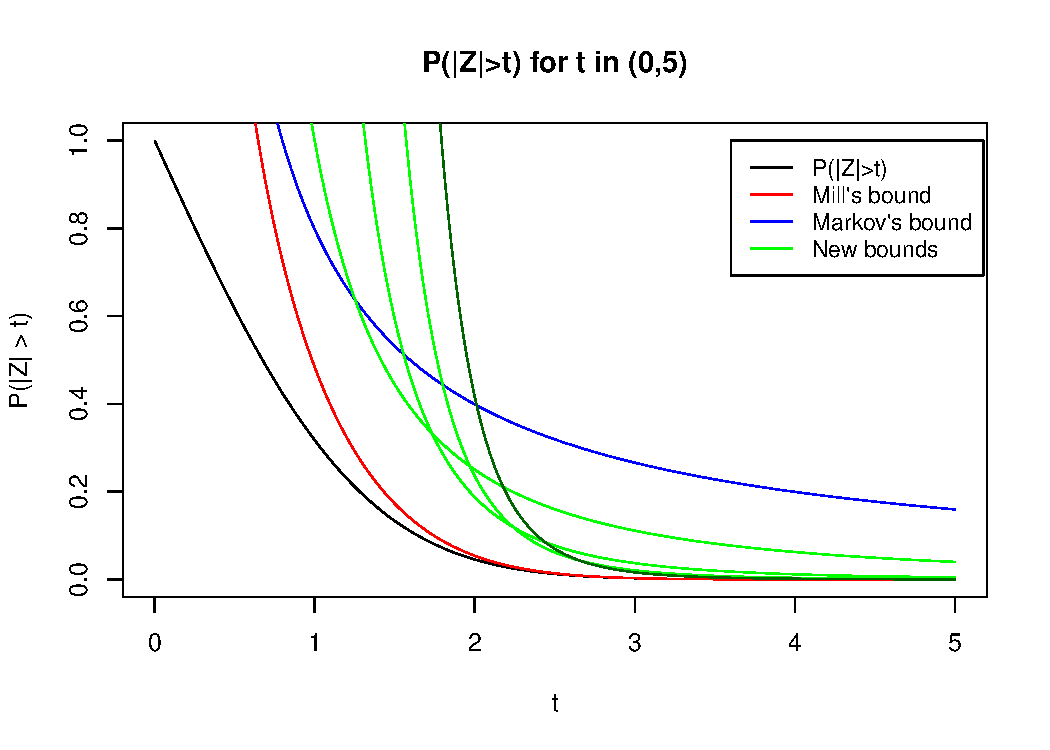
\includegraphics[scale=0.7]{ch5_10.pdf}
\end{figure}
Code for making this plot is in \texttt{5.10.R}.



\newpage\noindent
%%%%%%%%%%%%%%%%%%%%%%%%%%%%%%%%%%%%%%%%%%%%%%%%%%%%%%%%%%%%%%%%%%%%%%%%%%%%%%%
\textbf{5.11}\\  % PDF page 84
Let $X_n\sim N(0, 1/n)$ and let $X$ have the following CDF:
$$
F(x) =
\left\{
    \begin{tabular}{ll}
        0 & $x<0$ \\
        1 & $x\geq 0$
    \end{tabular}
\right.
$$
The variable $X$ has a point mass distribution at 0, and we want to see if
$X_n$ converges. Note that $\mu = \E[X_n] = 0$ and $\sigma^2 = \V(X_n) = 1/n$
and $\lim_{n\ra\infty}(1/n) = 0$, so by 5.2, this actually converges in quadratic
mean to 0, which implies convergence in distribution.

Also showing it directly by using Chebyshev's inequality. For any $\eps > 0$:
$$
\P(|X_n - 0| > \eps) \leq \frac{\sigma^2}{\eps^2} = \frac{1}{n\eps^2} \ra  0
$$
when $n\ra\infty$. In conclusion, $X_n\raP X$.

Next is investigating convergence in distribution which must be true, since convergence
in probability implies convergence in distribution. We can also see the trend by
plotting the CDF of $X_n$ for $n=1, 2, 5, 10, \ldots, 5000$ where $n=5000$ is in black.
Code for generating plot in \texttt{5.11.R}.
\begin{figure}[H]
    \centering
    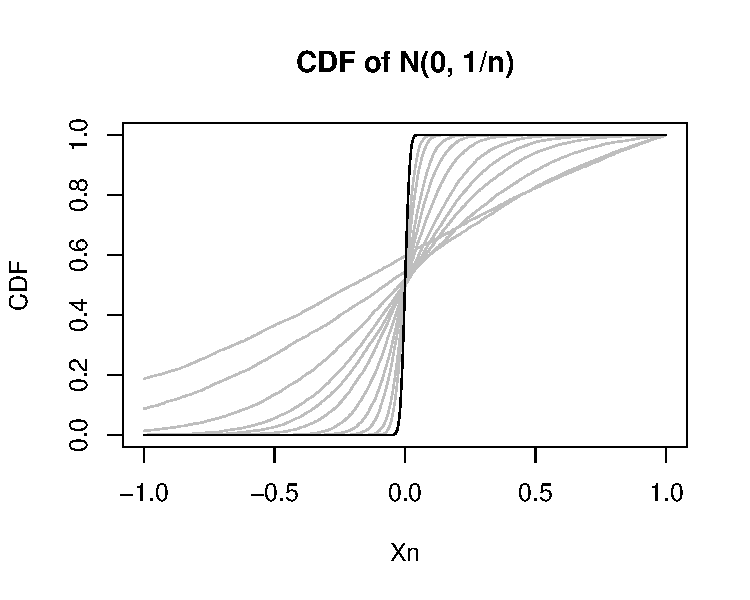
\includegraphics[scale=0.8]{ch5_11.pdf}
\end{figure}
To show convergence in distribution, we find an expression for the CDF of $X_n$.
By using the definition of the CDF and translating to the standard normal distribution:
$$
F_n(z) = \P(X\leq z) = \P\left(\frac{X_n - 0}{1/\sqrt{n}}\leq \frac{z - 0}{1/\sqrt{n}}\right)
= \P(\sqrt{n}X_n \leq \sqrt{n}z) = \P(Z\leq \sqrt{n}z),
$$
where $Z\sim N(0,1)$. As $n\ra\infty$ then for any $z<0$, $F_n(z) = 0$ and for $z\geq 0$
$F_n(z) = 1$ so it assumes the exact same form as $F(x)$, so $F_n\ra F$ and $X_n\raD X$
as $n\ra\infty$.

\newpage\noindent
%%%%%%%%%%%%%%%%%%%%%%%%%%%%%%%%%%%%%%%%%%%%%%%%%%%%%%%%%%%%%%%%%%%%%%%%%%%%%%%
\textbf{5.12}\\  % PDF page 84
Let $X_1,X_2,\ldots$ and $X$ be random variables that are positive integers.
Show that $X_n\raD X$ if and only if, for every integer $k$,
$$
\lim_{n\ra\infty} \P(X_n = k) = \P(X = k).
$$
\textsc{Proof}. This is a discrete random variable.\\
$\Rightarrow$). Assuming that $X_n\raD X$. By definition of convergence in distribution,
for any $k$,
$$
\lim_{n\ra\infty} F_n(k) = F(k)
\quad\text{and}\quad
\lim_{n\ra\infty} F_n(k-1) = F(k-1)
$$
Since we have a discrete distribution,
\begin{align*}
    F(k) - F(k-1)
    &= \sum_{p\leq k}\P(X=p) - \sum_{p\leq k-1}\P(X=p) \\
    &= \P(X=k) + \sum_{p\leq k-1}\P(X=p) - \sum_{p\leq k-1}\P(X=p) \\
    &= \P(X=k)
\end{align*}
The same relation is true for $F_n$, but here we also apply our assumption of convergence.
\begin{align*}
    \lim_{n\ra\infty}\P(X_n=k) &= \lim_{n\ra\infty}F_n(k) - \lim_{n\ra\infty}F_n(k-1) \\
    &= F(k) - F(k-1)
\end{align*}
By combining these together, we have shown, for any $k$,
$$
\lim_{n\ra\infty}\P(X_n=k) = \P(X=k).
$$
$\Leftarrow$) Now we assume that the limit of $\P(X_n = k)$ is equal to $\P(X = k)$ for all $k$,
which means they have equal probability mass function. Then, for any $k$:
\begin{align*}
    F(k) &= \P(X\leq k) = \sum_{z=1}^k\P(X = z) \\
    &= \P(X = 1) + \P(X = 2) + \ldots + \P(X = k) \\
    &= \lim_{n\ra\infty}\P(X_n = 1) + \lim_{n\ra\infty}\P(X_n = 2) + \ldots + \lim_{n\ra\infty}\P(X_n = k) \\
    &= \sum_{z=1}^k\lim_{n\ra\infty}\P(X_n = z) \\
    &= \lim_{n\ra\infty}\sum_{z=1}^k\P(X_n = z) \\
    &= \lim_{n\ra\infty} \P(X_n\leq k) = \lim_{n\ra\infty} F_n(k)
\end{align*}
(We can change the order of the sum and limit since it is a finite sum).
In conclusion, this shows that $\lim_{n\ra\infty} F_n(k) = F(k)$ and so $X_n\raD X$.\qed

\bigskip\noindent
%%%%%%%%%%%%%%%%%%%%%%%%%%%%%%%%%%%%%%%%%%%%%%%%%%%%%%%%%%%%%%%%%%%%%%%%%%%%%%%
\textbf{5.13}\\  % PDF page 84
Let $Z_1,Z_2,\ldots$ be IID random variables with density $f$. Suppose
$\P(Z_i > 0) = 1$ and that $\lim_{x\downarrow 0}f(x) > 0$ Define:
$$
X_n = n\min\{Z_1,\ldots, Z_n\}.
$$
Show that $X_n\raD Z$ where $Z\sim\text{Exp}(1/\lambda)$.


\begin{comment}

\bigskip\noindent
%%%%%%%%%%%%%%%%%%%%%%%%%%%%%%%%%%%%%%%%%%%%%%%%%%%%%%%%%%%%%%%%%%%%%%%%%%%%%%%
\textbf{5.X}\\  % PDF page 84


\begin{align*}
    A &= B
\end{align*}


\begin{equation*}
    A = B
    \tag*{\qed}
\end{equation*}


\begin{lstlisting}[style=RSyntax, title=R]
# Code
\end{lstlisting}

\begin{verbatim}
# Output
\end{verbatim}






%%%%%%%%%%%%%%%%%%%%%%%%%%%%%%%%%%%%%%%%%%% Minipages x 2
\begin{figure}[H]
    \begin{minipage}{0.5\textwidth}
        % MINIPAGE 1
    \end{minipage}
    \begin{minipage}{0.5\textwidth}
        % MINIPAGE 2
    \end{minipage}
\end{figure}

%%%%%%%%%%%%%%%%%%%%%%%%%%%%%%%%%%%%%%%%%%% Two R images
\begin{figure}[H]
    \begin{minipage}{0.5\textwidth}
    \begin{center}
        \begin{figure}[H]
            \includegraphics[scale=0.7]{IMG1.pdf}
        \end{figure}
    \end{center}
    \end{minipage}
    \begin{minipage}{0.5\textwidth}
    \begin{center}
        \begin{figure}[H]
            \includegraphics[scale=0.7]{IMG2.pdf}
        \end{figure}
    \end{center}
    \end{minipage}
\end{figure}


%%%%%%%%%%%%%%%%%%%%%%%%%%%%%%%%%%%%%%%%%%% Two TikZ images
%%% Tikz Image - side by side
\begin{figure}
    \begin{minipage}[0.5\textwidth]
\begin{tikzpicture}
    \begin{axis}[
        width=\textwidth,
        axis lines = left,
        ymin = -0.002,
        ymax = 2.1,
        xlabel = $z$,
        ylabel = {$f_Z(z)$},
    ]
    %Section 1
    \addplot [
        domain=0:1, 
        samples=10, 
        color=blue,
        style=ultra thick,
    ]
    {2 - 2*x};
    \end{axis}
\end{tikzpicture}
    \end{minipage}
    \begin{minipage}[0.5\textwidth]
\begin{tikzpicture}
    \begin{axis}[
        width=\textwidth,
        axis lines = left,
        ymin = -0.002,
        ymax = 2.1,
        xlabel = $z$,
        ylabel = {$f_Z(z)$},
    ]
    %Section 1
    \addplot [
        domain=0:1, 
        samples=10, 
        color=blue,
        style=ultra thick,
    ]
    {2 - 2*x};
    \end{axis}
\end{tikzpicture}
    \end{minipage}
\end{figure}
    
    
    
\end{comment}